Handler om at sikre de data der sendes mellem systems på LAN netværk og internettet, så det ikke kan læses af uvedkommende.

\section{Kryptografi}
\begin{itemize}
	\item Plaintext/cleartext = Ukrypteret besked
	\item Ciphertext = Krypteret besked
\end{itemize}


\subsection{Symmetrisk}
\begin{itemize}
	\item Samme nøgle benyttes til kryptering/dekryptering.
	\item Caesar Cipher
	\item Monoalphabetic cipher
\end{itemize}

{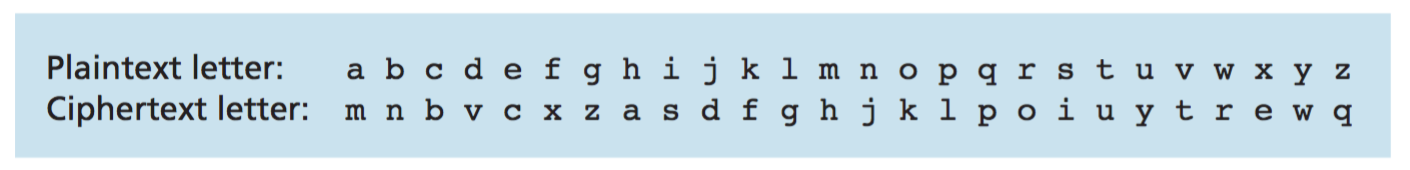
\includegraphics[scale=0.7]{8-security-overview/monoalphabetic.png}

\subsection{Asymmetrisk}
\begin{itemize}
	\item RSA Algoritmen (Navngivet efter opfinderne.)
	\item Private key / public key.
\end{itemize}

{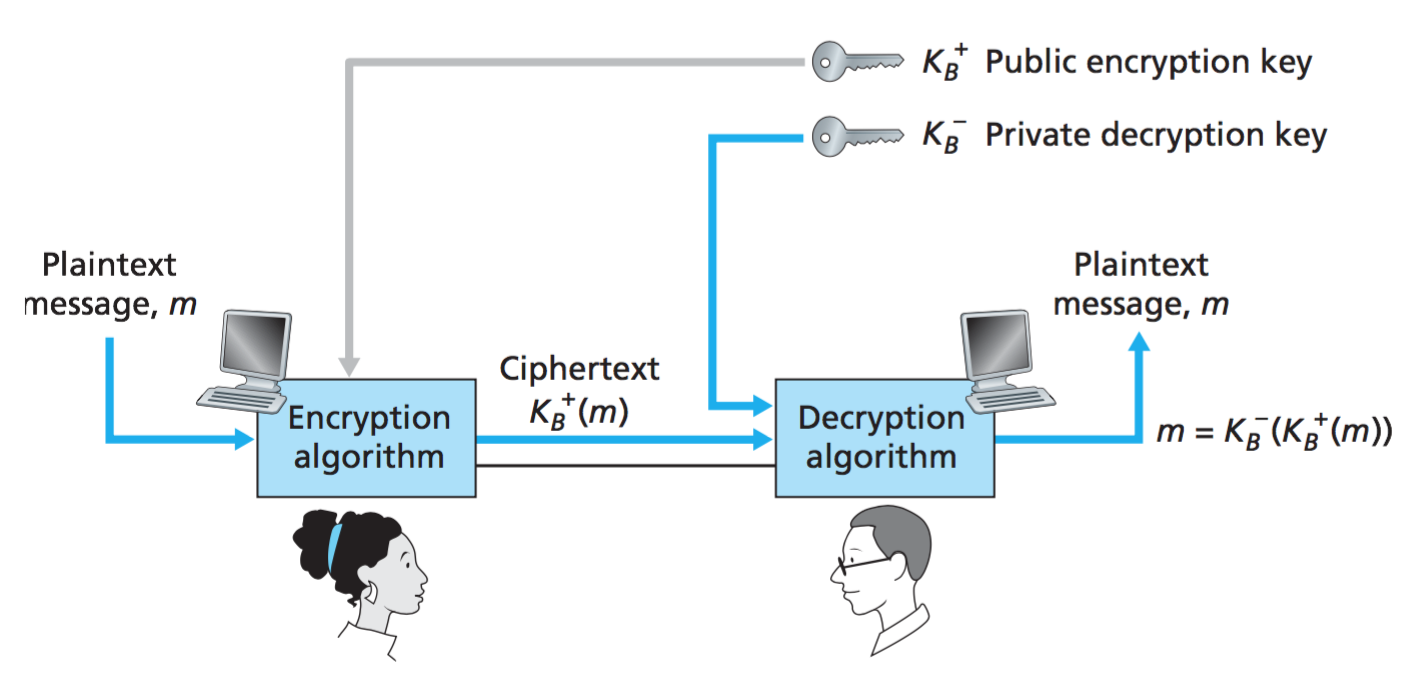
\includegraphics[scale=0.7]{8-security-overview/public-key-cryptography.png}


\subsection{Integritet}
\begin{itemize}
	\item Verificere at beskeden kommer fra den korrekte afsender.
	\item Verificere at beskeden ikke er blevet manipuleret undervejs.
\end{itemize}

\subsection{Hashing}
\begin{itemize}
	\item Vis størrelse er foretrukken for at undgå hashing kollision.
	\item Det skal ikke kunne betale sig, at forsøge at knække koden.
\end{itemize}

\subsection{Digital Signatur}
\begin{itemize}
	\item En digital erstatning for den fysiske signatur.
	\item Benytter public key kryptografi.
\end{itemize}
{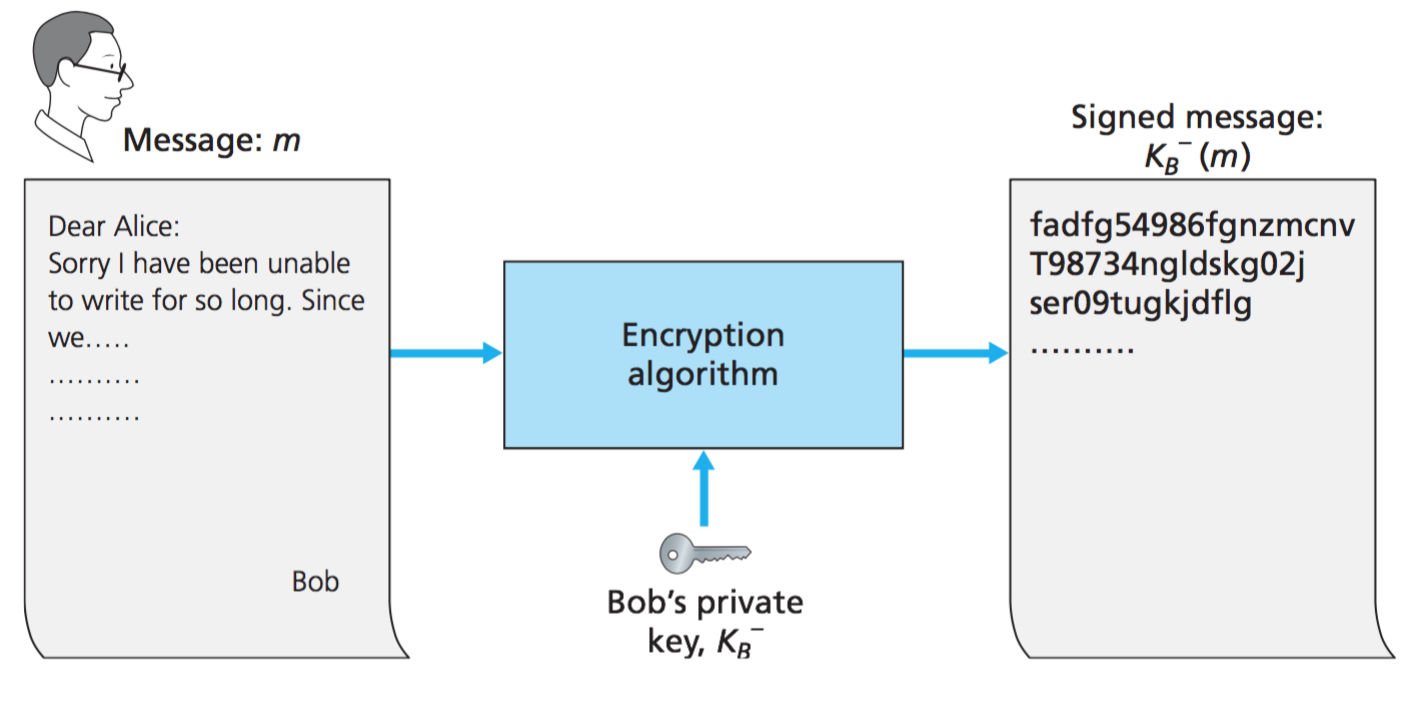
\includegraphics[scale=0.7]{8-security-overview/digital-signature.png}

\subsection{End-point authentication}
\begin{itemize}
	\item En entitet beviser dens identitet overfor en anden entitet på et computer netværk.
	\item Fx: bruger beviser identitet overfor en mailserver.
\end{itemize}

{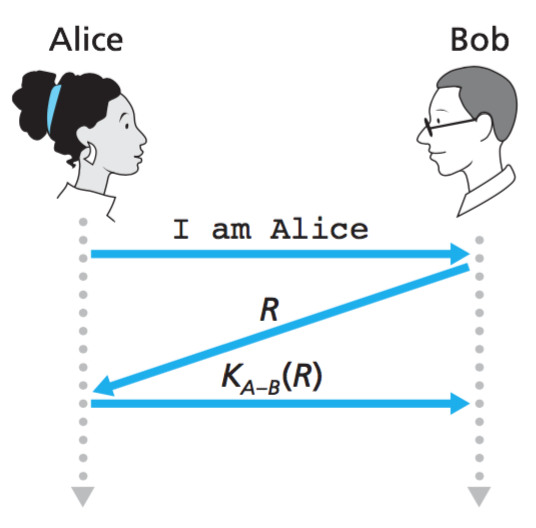
\includegraphics[scale=0.9]{8-security-overview/endpoint.png}

\subsection{SSL}

\begin{itemize}
	\item Kryptografi kan forbedre TCP med henblik på sikkerhedsmæssige aspekter.
	\item Fortrolighed, data-integritet og end point authentication.
	\item Certifikat købes igennem en 3.partsudbyder og installeres på webserver. Består af en public og private key.
	\item TLS (Transport Layer Security) er en modificeret version af SSL.
\end{itemize}

\subsection{IPsec}
\begin{itemize}
	\item IP Security Protocol.
	\item Står for sikkerhed for netværks lag.
	\item Verificering/Kryptering af hver IP-datagram.
	\item Beskytter data flows mellem et host-par: (Host-to-Host, network-to-host, network-to-network).
\end{itemize}

